\documentclass[11pt,a4paper]{article}

% ------------------------------------------------------------
% Multi-Agent Systems and Agentic AI practical examination
% LaTeX report template
% ------------------------------------------------------------
% Required format from coursework brief:
% - A4 paper
% - 11 pt body font
% - Single column
% - Margins of at least 2 cm
% - Single line spacing
% - Single PDF covering both parts
% - Section I.4 must be typeset in LaTeX
% - Every URL must be clickable
% ------------------------------------------------------------

\usepackage[a4paper,margin=2cm]{geometry}
\usepackage{setspace}
\singlespacing

\usepackage[T1]{fontenc}
\usepackage[utf8]{inputenc}
\usepackage{lmodern}
\usepackage[british]{babel}
\usepackage{microtype}

\usepackage{amsmath,amssymb,mathtools,bm}
\usepackage{graphicx}
\usepackage{booktabs}
\usepackage{array}
\usepackage{enumitem}
\usepackage{xcolor}
\usepackage{caption}
\usepackage{subcaption}
\usepackage{float}
\usepackage{tikz}
\usetikzlibrary{arrows.meta,positioning,shapes.geometric,fit}

\usepackage[hidelinks]{hyperref}
\usepackage[nameinlink,noabbrev]{cleveref}

% ------------------------------------------------------------
% Helpful commands
% ------------------------------------------------------------
\newcommand{\code}[1]{\texttt{#1}}
\newcommand{\repo}{\href{https://gitlab.developers.cam.ac.uk/YOUR-CRSID/YOUR-REPO}{GitLab repository}}
\newcommand{\wandb}{\href{https://wandb.ai/YOUR-PROJECT/YOUR-RUN}{W\&B run}}
\newcommand{\cmbcommit}{\href{https://github.com/borisbolliet/cmbagent_lg/tree/adaptive-planning}{cmbagent\_lg adaptive-planning branch}}
\newcommand{\TODO}[1]{\textcolor{red}{[TODO: #1]}}

\setlist[itemize]{leftmargin=*,topsep=2pt,itemsep=1pt}
\setlist[enumerate]{leftmargin=*,topsep=2pt,itemsep=1pt}

% Keep tables compact by default
\renewcommand{\arraystretch}{1.12}

% ------------------------------------------------------------
% Metadata
% ------------------------------------------------------------
\title{Multi-Agent Systems and Agentic AI\\Practical Examination Report}
\author{Frederick Lawrence \\ CRSid: fl482 \\ Team members for Part I: Name 1, Name 2}
\date{\today}

\begin{document}

\maketitle

\noindent\textbf{Repository and logs.}
The code used for Part I is available at \repo. Training and evaluation logs are available at \wandb. The adaptive-planning implementation studied in Part II is linked at \cmbcommit. Replace these placeholders with exact clickable URLs, including the exact commit where required.

\vspace{0.5em}
\noindent\textbf{Notes on jointly owned work.}
Sections I.1--I.3 describe experiments run using the shared team TPU and shared repository. The analysis and prose in this report are my own. Section I.4 and Part II are completed individually.

\tableofcontents
\newpage

% ============================================================
\section*{Part I: GRPO finetuning of Gemma 3 on a TPU}
\addcontentsline{toc}{section}{Part I: GRPO finetuning of Gemma 3 on a TPU}
% Sections I.1--I.3 together should be at most 3 pages, excluding references and appendix.
% I.4 has no page limit, but should be clear and concise.

\subsection*{I.1 Reproducing the baseline}
\addcontentsline{toc}{subsection}{I.1 Reproducing the baseline}

\paragraph{Run details.}
\begin{table}[H]
    \centering
    \caption{Baseline run details.}
    \label{tab:baseline-run-details}
    \begin{tabular}{ll}
        \toprule
        Item & Value \\
        \midrule
        Repository commit & \code{TODO} \\
        TPU type & v6e-1 \\
        Training command & \code{python scripts/train.py} \\
        Evaluation command & \code{python scripts/evaluate.py} \\
        Wall-clock time & \TODO{e.g. 6 h 20 min} \\
        GRPO steps completed & \TODO{number of steps} \\
        Held-out split & \TODO{e.g. GSM8K test split} \\
        Evaluation seed & \TODO{fixed seed} \\
        \bottomrule
    \end{tabular}
\end{table}

\paragraph{Baseline patches.}
\TODO{State whether the baseline ran as shipped. If not, document the minimal fix required, with the affected file and commit. Keep this short.}

\paragraph{Evaluation.}
\begin{table}[H]
    \centering
    \caption{Baseline GSM8K accuracy.}
    \label{tab:baseline-accuracy}
    \begin{tabular}{lccc}
        \toprule
        Model & Split & Seed & Accuracy \\
        \midrule
        Base model, \code{google/gemma-3-1b-it} & \TODO{split} & \TODO{seed} & \TODO{value} \\
        LoRA GRPO checkpoint & \TODO{split} & \TODO{seed} & \TODO{value} \\
        \bottomrule
    \end{tabular}
\end{table}

\begin{figure}[H]
    \centering
    \includegraphics[width=0.82\linewidth]{figures/baseline_reward_kl.pdf}
    \caption{Baseline training curves showing mean reward $\bar r$ and $\mathrm{KL}(\pi_\theta\|\pi_{\mathrm{ref}})$ against GRPO step.}
    \label{fig:baseline-reward-kl}
\end{figure}

\subsection*{I.2 Understanding the baseline}
\addcontentsline{toc}{subsection}{I.2 Understanding the baseline}
% This subsection should be at most one page.

\paragraph{Policies in the LoRA setup.}
\TODO{Explain what plays the role of $\pi_\theta$, $\pi_{\mathrm{old}}$ and $\pi_{\mathrm{ref}}$, and identify which carries trainable parameters.}

\paragraph{Group size and advantage estimator.}
\TODO{State the group size $K$ from \code{scripts/config.py}. Identify the Tunix advantage estimator and state whether it is standard group-mean or leave-one-out.}

\paragraph{Reward terms.}
\TODO{Identify shaping rewards and the true correctness reward in \code{scripts/rewards.py}. Explain what would happen early in training with correctness reward alone in terms of within-group reward variance $\sigma_r$.}

\paragraph{Clipped surrogate.}
\TODO{Locate where the PPO-style clipped surrogate is implemented in Tunix. State what $\varepsilon$ corresponds to in \code{scripts/config.py} and note any deviation from the lecture form, such as per-token rather than per-sequence ratios.}

\subsection*{I.3 Improving on the baseline}
\addcontentsline{toc}{subsection}{I.3 Improving on the baseline}

\paragraph{Modification and motivation.}
\TODO{Describe the principled modification. Examples: leave-one-out advantage, sweep $K$, change $\beta$ or $\varepsilon$, modify shaping rewards, add length penalty, change LoRA rank, learning rate, schedule or generation length. Connect the choice to GRPO theory.}

\paragraph{Controlled comparison.}
\TODO{State how the comparison was controlled: same data, same evaluation split, same total compute or normalised per step. Mention baseline plus at least two further complete runs, or justify fewer.}

\begin{table}[H]
    \centering
    \caption{Controlled comparison on held-out GSM8K. Include uncertainty using a second seed or a bootstrap confidence interval over evaluation prompts.}
    \label{tab:controlled-comparison}
    \begin{tabular}{lcccc}
        \toprule
        Model / run & Modification & Seed(s) & Accuracy & Uncertainty \\
        \midrule
        Base model & None & \TODO{} & \TODO{} & \TODO{} \\
        Baseline GRPO & Default config & \TODO{} & \TODO{} & \TODO{} \\
        Variant 1 & \TODO{} & \TODO{} & \TODO{} & \TODO{} \\
        Variant 2 & \TODO{} & \TODO{} & \TODO{} & \TODO{} \\
        \bottomrule
    \end{tabular}
\end{table}

\begin{figure}[H]
    \centering
    \includegraphics[width=0.82\linewidth]{figures/reward_kl_variants.pdf}
    \caption{Training curves for the baseline and variants on shared axes, showing mean reward and KL over GRPO step.}
    \label{fig:reward-kl-variants}
\end{figure}

\begin{figure}[H]
    \centering
    \includegraphics[width=0.82\linewidth]{figures/grpo_diagnostic.pdf}
    \caption{Diagnostic plot for a known GRPO failure mode, such as advantage distribution, degenerate reward groups, response length, entropy, or KL versus accuracy.}
    \label{fig:grpo-diagnostic}
\end{figure}

\paragraph{Discussion.}
\TODO{Connect the empirical findings to lecture theory. State whether the observed behaviour matched the prediction, and diagnose any negative results honestly.}

\subsection*{I.4 GRPO theory}
\addcontentsline{toc}{subsection}{I.4 GRPO theory}
% This section must be written in LaTeX. There is no page limit, but verbosity is penalised.
% Use amsmath environments and number equations that you refer back to.

\subsubsection*{Question 1}
\addcontentsline{toc}{subsubsection}{Question 1}

\paragraph{(i)}
\TODO{Compute $\mathbb{E}[X_i]$ and hence $\mathbb{E}[\hat g]$. Explain why zero expectation in this fixed-response setup does not imply that the underlying policy gradient vanishes.}

\paragraph{(ii)}
\TODO{Identify the shared random term and compute $\operatorname{Cov}(X_i,X_j)$ for $i\neq j$.}

\paragraph{(iii)}
\TODO{Compute $\operatorname{Var}(\hat g)$ and compare it with the naive iid scaling. Define an effective sample size $K_{\mathrm{eff}}$.}

\subsubsection*{Question 2}
\addcontentsline{toc}{subsubsection}{Question 2}

\paragraph{(i)}
\TODO{Derive the unique optimiser of the KL-regularised update and interpret $\eta$.}

\paragraph{(ii)}
\TODO{Show monotone improvement under exact advantage and identify a practical failure condition for GRPO with neural networks.}

\paragraph{(iii)}
\TODO{Describe the trust region induced by PPO-style clipping and contrast it with a joint KL constraint.}

\subsubsection*{Question 3}
\addcontentsline{toc}{subsubsection}{Question 3}

\paragraph{(i)}
\TODO{Derive the importance-corrected estimator under $\pi_{\mathrm{mix}}$ and give $w_i$.}

\paragraph{(ii)}
\TODO{Verify the $\alpha\to 0$ limit.}

\paragraph{(iii)}
\TODO{Express $V^{\pi_{\mathrm{mix}}}(q)$ and derive the reweighted advantage needed to avoid baseline shift.}

\paragraph{(iv)}
\TODO{Compare the variance of $\hat g_{\mathrm{mix}}$ and $\hat g_{\mathrm{GRPO}}$ under conditions where uniform mixing increases or decreases variance.}

\paragraph{(v)}
\TODO{Explain weight collapse for long responses and propose a concrete fix with its trade-off.}

% ============================================================
\section*{Part II: Adaptive planning in \code{cmbagent\_lg}}
\addcontentsline{toc}{section}{Part II: Adaptive planning in cmbagent\_lg}
% Part II should be at most 2 pages, excluding the workflow diagram.

\subsection*{II.1 Workflow diagram}
\addcontentsline{toc}{subsection}{II.1 Workflow diagram}

\begin{figure}[H]
    \centering
    % Replace this TikZ sketch with the final workflow diagram once the implementation has been studied.
    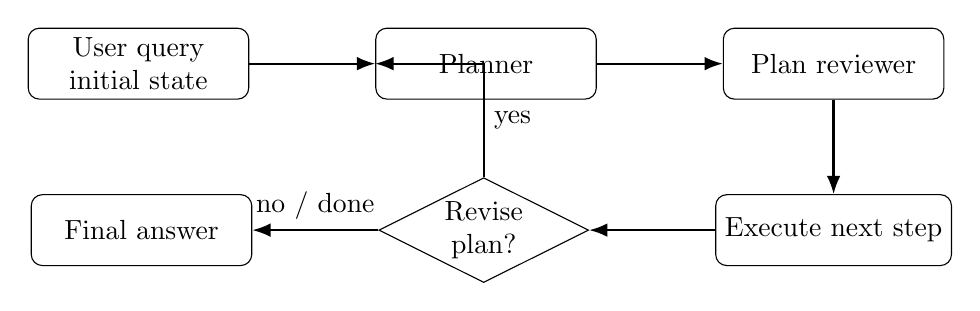
\begin{tikzpicture}[
        node distance=1.2cm and 1.6cm,
        box/.style={draw,rounded corners,align=center,minimum width=2.8cm,minimum height=0.9cm},
        decision/.style={draw,diamond,aspect=2,align=center,inner sep=1pt},
        arrow/.style={-Latex,thick}
    ]
        \node[box] (input) {User query\\initial state};
        \node[box,right=of input] (planner) {Planner};
        \node[box,right=of planner] (reviewer) {Plan reviewer};
        \node[box,below=of reviewer] (execute) {Execute next step};
        \node[decision,left=of execute] (adapt) {Revise\\plan?};
        \node[box,left=of adapt] (finish) {Final answer};

        \draw[arrow] (input) -- (planner);
        \draw[arrow] (planner) -- (reviewer);
        \draw[arrow] (reviewer) -- (execute);
        \draw[arrow] (execute) -- (adapt);
        \draw[arrow] (adapt) -- node[above]{no / done} (finish);
        \draw[arrow] (adapt) |- node[pos=0.25,right]{yes} (planner);
    \end{tikzpicture}
    \caption{Placeholder adaptive-planning workflow. Replace this with the exact LangGraph nodes, edges, conditional routing, and state fields from the studied commit. This diagram does not count towards the 2-page Part II limit.}
    \label{fig:adaptive-planning-workflow}
\end{figure}

\paragraph{Walkthrough.}
\TODO{In at most half a page, explain what triggers a plan revision, what part of the plan may change, what is held fixed across a revision, and how the loop terminates. Include the exact commit link studied.}

\subsection*{II.2 Problems}
\addcontentsline{toc}{subsection}{II.2 Problems}

\paragraph{Problem 1: \TODO{short name}.}
\TODO{Argue the limitation or failure mode, grounded in planning and closed-loop control theory.}

\paragraph{Problem 2: \TODO{short name}.}
\TODO{Argue the limitation or failure mode, grounded in planning and closed-loop control theory.}

\paragraph{Problem 3: \TODO{short name}.}
\TODO{Argue the limitation or failure mode, grounded in planning and closed-loop control theory.}

\subsection*{II.3 Proposed improvements}
\addcontentsline{toc}{subsection}{II.3 Proposed improvements}

\paragraph{Improvement 1.}
\TODO{State what changes, why it addresses the corresponding problem, and what it trades off.}

\paragraph{Improvement 2.}
\TODO{State what changes, why it addresses the corresponding problem, and what it trades off.}

\paragraph{Improvement 3.}
\TODO{State what changes, why it addresses the corresponding problem, and what it trades off.}

% ============================================================
\newpage
\section*{References}
\addcontentsline{toc}{section}{References}
% References do not count towards the page limits.
% Replace this manual list with biblatex or BibTeX if preferred.

\begin{itemize}
    \item Hu, E. J. et al. (2021). \emph{LoRA: Low-Rank Adaptation of Large Language Models}. \url{https://arxiv.org/abs/2106.09685}
    \item Tunix documentation or source link used for GRPO implementation: \url{https://github.com/google/tunix}
    \item Exact \code{cmbagent\_lg} adaptive-planning commit studied: \TODO{insert clickable commit URL}
\end{itemize}

\appendix
\section{Appendix}
% Appendices do not count towards the page limits but must not contain material essential to marking.

\subsection{Additional run details}
\TODO{Optional non-essential logs, extra tables, hyperparameter dumps, and supplementary figures.}

\end{document}
